\documentclass{beamer}
\usetheme{Madrid}
\usepackage{tikz}
\usepackage{amsmath}
\usetikzlibrary{calc}

\title{Visualizing Loss Landscapes}
\author{T.N.}
\date{}

\begin{document}

\begin{frame}{Loss Landscape}
    \begin{figure}
        \centering
        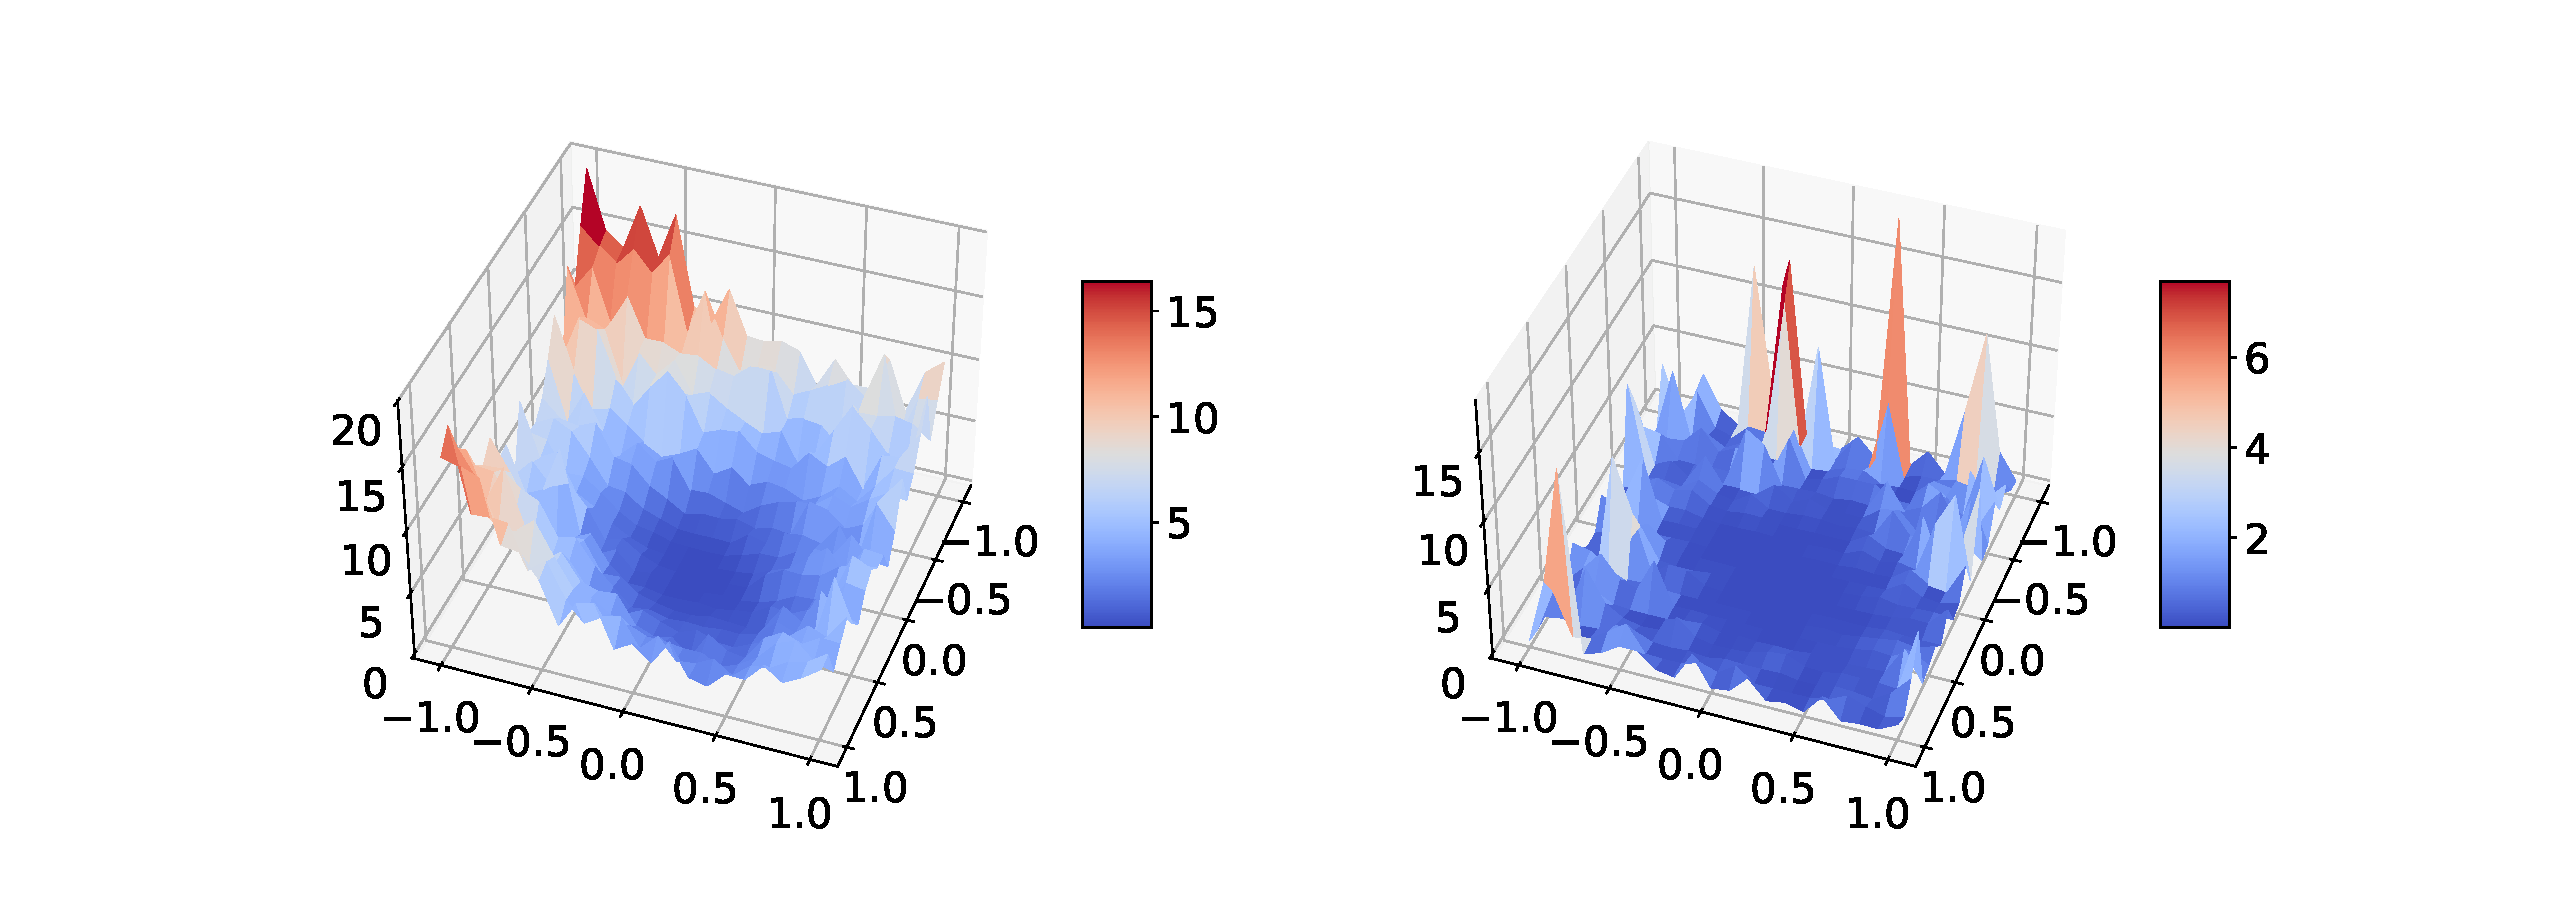
\includegraphics[width=1.86\textwidth]{loss_eigen_1_2.pdf}
    \end{figure}
\end{frame}

% Slide 1
\begin{frame}{Loss Landscape \(\Leftrightarrow\) Mountain Range}
    \begin{columns}[T,onlytextwidth]
        \begin{column}{0.48\textwidth}
            \textbf{Loss Surface}
            \begin{itemize}
                \item Sharp peaks \(\rightarrow\) high curvature directions
                \item Valleys \(\rightarrow\) local minima
            \end{itemize}

            \vspace{1em}
            \textbf{Projection onto Dominant Eigen-Directions}
            \begin{itemize}
                \item Hessian eigenvectors: principal axes
                \item \(\Delta_k\): metric of landscape change
            \end{itemize}
        \end{column}

        \begin{column}{0.48\textwidth}
            \textbf{Mountain Range}
            \begin{itemize}
                \item Sharp peaks \(\rightarrow\) steep slopes
                \item Valleys \(\rightarrow\) low points
            \end{itemize}

            \vspace{1em}
            \textbf{Drone Sampling}
            \begin{itemize}
                \item \(\Delta_k\): volume of sampled points
                \item Provides “terrain” measurements
            \end{itemize}
        \end{column}
    \end{columns}

    % Dashed arrow connecting the two concepts
    \begin{tikzpicture}[overlay, remember picture]
        % Define start and end points relative to frame
        \coordinate (start) at ($(current page.north west) + (3.5cm,-2cm)$);
        \coordinate (end)   at ($(current page.north east) + (-3.5cm,-2cm)$);
        \draw[dashed, ->, thick] (start) -- node[above]{\(\Delta_k\) (drone sampling)} (end);
    \end{tikzpicture}
\end{frame}

\end{document}
